\documentclass[letterpaper]{article}

\usepackage{geometry}
\newgeometry{vmargin={25mm}, hmargin={30mm,30mm}}

\setcounter{secnumdepth}{0}

\usepackage{noto}
\usepackage{CJKutf8}
\usepackage[T1]{fontenc}

\usepackage{amsmath}
\usepackage{listings}
\usepackage{xcolor}
\usepackage{multirow}
\usepackage{float,graphicx}
\usepackage{subcaption}
\usepackage[breaklinks=true]{hyperref}
\usepackage{etoolbox}
\appto\UrlBreaks{\do\-}

\usepackage{mdframed}
\newenvironment{modeloutput}[1]{%
	\begin{mdframed}[backgroundcolor=gray!8, linecolor=gray!60, linewidth=0.8pt,
		innerleftmargin=8pt, innerrightmargin=8pt, innertopmargin=6pt, innerbottommargin=6pt]%
		\small\ttfamily\raggedright
	}{%
	\end{mdframed}%
}

\lstset{
	basicstyle=\small\ttfamily,
	tabsize=4,
	frame=single,
	breaklines,
	postbreak=\mbox{\textcolor{red}{$\hookrightarrow$}\space},
	showstringspaces=false,
}

\newcommand{\repofile}[2]{\href{https://github.com/echung32/ece405-assignment4-hpc/blob/main/#1}{#2}}
\newcommand{\todo}[1]{\textbf{TODO:} #1}
\graphicspath{{report/figures/}{figures/}}

\begin{document}
	\title{Assignment 4: Systems and Parallelism}
	
	\author{Ethan Chung\\
		{\tt\small University of Hawaii}\\
		{\tt\small ECE 405: Intro to Large-Scale AI Systems}\\
		{\tt\small [redacted]@hawaii.edu}}
	
	\maketitle
	
	\tableofcontents
	
	\newpage
	
	\section{Profiling and Benchmarking}
	
	\subsection{Problem (benchmarking\_script): 4 points}
	
	\begin{itemize}
		\item[(a)] Write a script to perform basic end-to-end benchmarking of the forward and backward passes in your model.
		
		\textit{Implemented in \repofile{cs336_systems/section1/benchmarking_script.py}{cs336\_systems/section1/benchmarking\_script.py}.}
		
		\item[(b)] Time the forward and backward passes for the model sizes described in the assignment using 5 warmup steps and 10 measured steps. How long does a forward pass take? How about a backward pass? Do you see high variability across measurements, or is the standard deviation small?
		
		% All runs use batch size~1, FP32 precision, 5 warmup steps, and 10 measurement steps on a single GPU.
		Table~\ref{tab:fwd-timing} reports forward-only timings and Table~\ref{tab:fwdbwd-timing} reports forward + backward timings (mean $\pm$ standard deviation in ms).
		
		\begin{table}[H]
			\centering
			\caption{Forward-only timing (FP32, mean $\pm$ std, ms)}
			\label{tab:fwd-timing}
			\begin{tabular}{lrrrr}
				\hline
				Model & ctx=128 & ctx=256 & ctx=512 & ctx=1024 \\
				\hline
				small  & $13.1 \pm 0.4$  & $13.7 \pm 2.1$  & $16.9 \pm 1.8$  & $27.4 \pm 6.6$ \\
				medium & $25.7 \pm 1.1$  & $27.0 \pm 2.3$  & $40.7 \pm 5.6$  & $69.8 \pm 1.2$ \\
				large  & $42.8 \pm 2.7$  & $54.1 \pm 5.5$  & $121.4 \pm 4.1$ & $227.9 \pm 0.3$ \\
				xl     & $88.4 \pm 4.6$  & $90.4 \pm 3.6$  & $217.7 \pm 4.8$ & $500.9 \pm 56.6$ \\
				2.7B   & $159.4 \pm 6.7$ & $239.5 \pm 7.6$ & $298.5 \pm 7.1$ & $876.1 \pm 6.4$ \\
				\hline
			\end{tabular}
		\end{table}
		
		\begin{table}[H]
			\centering
			\caption{Forward + backward timing (FP32, mean $\pm$ std, ms)}
			\label{tab:fwdbwd-timing}
			\begin{tabular}{lrrrr}
				\hline
				Model & ctx=128 & ctx=256 & ctx=512 & ctx=1024 \\
				\hline
				small  & $30.6 \pm 2.1$   & $37.3 \pm 3.3$  & $51.9 \pm 2.5$   & $80.7 \pm 4.3$ \\
				medium & $64.6 \pm 6.5$   & $73.2 \pm 4.1$  & $119.9 \pm 0.8$  & $198.4 \pm 34.8$ \\
				large  & $112.6 \pm 1.2$  & $224.2 \pm 2.0$ & $349.4 \pm 4.8$  & $697.4 \pm 1.0$ \\
				xl     & $272.2 \pm 3.9$  & $406.1 \pm 4.8$ & $637.7 \pm 8.3$  & $1709.1 \pm 278.0$ \\
				2.7B   & $691.6 \pm 115.3$ & $759.6 \pm 9.5$ & $1474.5 \pm 174.8$ & $1835.2 \pm 315.8$ \\
				\hline
			\end{tabular}
		\end{table}
		
		Forward pass times range from about 13~ms (small, ctx=128) to 876~ms (2.7B, ctx=1024), while forward~+ backward is roughly 2--3$\times$ slower. Standard deviations are generally small (under 5\%) for smaller models but grow larger at the xl and 2.7B scales, especially at longer context lengths, likely due to memory pressure on the GPU.
		
		\item[(c)] Repeat the analysis without warm-up steps. How does this affect your results? Why do you think this happens? Also try to run the script with 1 or 2 warm-up steps. Why might the result still be different?
		
		Without warm-up steps, the all-steps mean at \(w{=}0\) is substantially inflated relative to the steady-state baseline \(w{=}5\), increasing from \(13.9\text{--}32.7\) ms to \(51.0\text{--}69.6\) ms for forward passes and from \(35.9\text{--}93.4\) ms to \(86.5\text{--}141.2\) ms for forward+backward passes. However, excluding only the first iteration produces steady-state timings at \(w{=}0\) that closely match the \(w{=}5\) results (e.g., \(15.4\) ms vs.\ \(14.0\) ms for forward, ctx \(=128\); \(92.6\) ms vs.\ \(93.1\) ms for forward+backward, ctx \(=1024\)), indicating that the overhead is concentrated almost entirely in the initial cold-start iteration. Similarly, \(w{=}1\) and \(w{=}2\) produce timings nearly identical to \(w{=}5\) across all context lengths and modes, suggesting that a single warm-up step is generally sufficient to remove most initialization overhead on this hardware.
		
		\begin{table}[h!]
			\centering
			\caption{Effect of warm-up steps on mean timing (ms) for the small model, FP32, batch size 1. ``Steady'' shows the mean of steps 2--10 only (excluding the cold-start first step).}
			\label{tab:warmup_comparison}
			\begin{tabular}{llrrrrrrrr}
				\hline
				& & \multicolumn{4}{c}{All-steps mean (ms)} & \multicolumn{4}{c}{Steady-state mean (ms)} \\
				Mode & ctx & $w{=}0$ & $w{=}1$ & $w{=}2$ & $w{=}5$ & $w{=}0$ & $w{=}1$ & $w{=}2$ & $w{=}5$ \\
				\hline
				Forward & 128  & \textbf{51.0}  & 14.8  & 14.3  & 13.9  & 15.4  & 14.9  & 14.2  & 14.0  \\
				Forward & 256  & \textbf{54.3}  & 15.7  & 14.0  & 14.4  & 15.5  & 15.3  & 14.1  & 14.3  \\
				Forward & 512  & \textbf{56.5}  & 18.0  & 19.8  & 18.5  & 17.9  & 18.0  & 20.1  & 18.7  \\
				Forward & 1024 & \textbf{69.6}  & 32.3  & 31.1  & 32.7  & 31.7  & 32.1  & 31.6  & 33.4  \\
				\hline
				Fwd+Bwd & 128  & \textbf{86.5}  & 35.1  & 34.1  & 35.9  & 33.7  & 34.6  & 33.6  & 35.9  \\
				Fwd+Bwd & 256  & \textbf{92.0}  & 40.2  & 39.6  & 38.8  & 41.0  & 40.9  & 39.8  & 38.3  \\
				Fwd+Bwd & 512  & \textbf{105.2} & 54.6  & 53.4  & 57.7  & 52.6  & 55.6  & 52.5  & 57.1  \\
				Fwd+Bwd & 1024 & \textbf{141.2} & 93.4  & 92.1  & 93.4  & 92.6  & 94.1  & 92.1  & 93.1  \\
				\hline
			\end{tabular}
		\end{table}
		
	\end{itemize}
	
	\subsection{Problem (nsys\_profile): 5 points}
	
	\begin{itemize}
		\item[(a)] Profile your forward pass, backward pass, and optimizer step using \texttt{nsys} for the required model sizes and context lengths. What is the total time spent on your forward pass? Does it match what we measured before with the Python standard library?
		
	Table~\ref{tab:nsys-vs-python} shows that the \texttt{nsys} NVTX forward-pass timings are generally within the same order of magnitude as the Python benchmark measurements, with the closest agreement observed for larger, compute-bound models and longer context lengths. Small-model, short-context runs show larger deviations because the shorter runtimes are more sensitive to cold-start overheads and scheduling variance relative to the total execution time.
		
		\begin{table}[H]
			\centering
			\caption{Forward-pass timing (ms): Python-timed benchmark (5 warmup, 10 steps) vs.\ \texttt{nsys} NVTX wall time (5 warmup, 1 step). FP32, batch size~1.}
			\label{tab:nsys-vs-python}
			\begin{tabular}{l|rr|rr|rr|rr}
				\hline
				& \multicolumn{2}{c|}{ctx=128} & \multicolumn{2}{c|}{ctx=256} & \multicolumn{2}{c|}{ctx=512} & \multicolumn{2}{c}{ctx=1024} \\
				Model & Py & nsys & Py & nsys & Py & nsys & Py & nsys \\
				\hline
				small  &  13.1 &  19.3 &  13.7 &  16.3 &  16.9 &  18.1 &  27.4 &  21.8 \\
				medium &  25.7 &  46.1 &  27.0 &  32.7 &  40.7 &  31.5 &  69.8 &  55.0 \\
				large  &  42.8 &  55.2 &  54.1 &  60.0 & 121.4 &  90.9 & 227.9 & 181.7 \\
				xl     &  88.4 &  72.1 &  90.4 &  66.9 & 217.7 &  88.9 & 500.9 & 324.4 \\
				2.7B   & 159.4 &  81.2 & 239.5 & 127.3 & 298.5 & 204.6 & 876.1 & 449.9 \\
				\hline
			\end{tabular}
		\end{table}
		
		\item[(b)] What CUDA kernel takes the most cumulative GPU time during the forward pass? How many times is this kernel invoked during a single forward pass of your model? Is it the same kernel that takes the most runtime when you do both forward and backward passes?
		
		The dominant forward-pass CUDA kernel is the GEMM kernel \texttt{cutlass\_80\_simt\_sgemm\_128x64\_8x5\_tn\_align1}, which accounts for 38\% of GPU kernel time and is invoked 36 times per forward step for the small model at ctx\(=128\). The same GEMM kernel family also dominates the full training step, although its fraction of total runtime decreases because AdamW introduces substantial elementwise optimizer overhead.
		
		\item[(c)] What other kernels besides matrix multiplies account for non-trivial CUDA runtime in the forward pass?
		
		Besides matrix multiplications, the main forward-pass kernels are \texttt{at::native::elementwise\_kernel} (7.7\%), \texttt{cublasLt::splitKreduce\_kernel} (7.2\%), and \texttt{at::native::index\_elementwise\_kernel} (3.4\%), corresponding to activations, GEMM reduction epilogues, and embedding lookups respectively. These kernels are primarily memory-bandwidth bound, which causes their runtime contribution to be disproportionately large relative to their FLOP count.
		
		\item[(d)] Profile one complete training step with AdamW. How does the fraction of time spent on matrix multiplication change compared to inference? How about other kernels?
		
		In the forward-only pass, GEMM kernels account for roughly 70\% of GPU kernel time, but this drops to 34\% during a full AdamW training step because optimizer elementwise update kernels contribute about 41\% of runtime. At longer context lengths, the GEMM fraction increases again (up to 58\%) as attention and feed-forward matrix multiplication costs grow with sequence length while optimizer cost remains fixed per parameter.
		
		\item[(e)] Compare the runtime of the softmax operation versus the matrix multiplication operations within the self-attention layer of your model during a forward pass. How does the difference in runtimes compare to the difference in FLOPs?
		
		Isolated \texttt{torch.profiler} measurements of a single attention head group (12 heads, $d_{\text{head}}=64$, ctx=128, 10 reps):
		\begin{itemize}
			\item QK matmul (\texttt{Q @ K\textsuperscript{T} / $\sqrt{d}$}): 7.6~\textmu s per call
			\item Softmax: 1.7~\textmu s per call
			\item AV matmul (\texttt{weights @ V}): 6.5~\textmu s per call
		\end{itemize}

		The softmax kernel takes approximately \(1.7~\mu s\) per call, compared to \(7.6~\mu s\) and \(6.5~\mu s\) for the QK and AV matrix multiplications respectively, making softmax only about \(4.5\times\) faster despite requiring roughly \(64\times\) fewer FLOPs. This discrepancy arises because the GEMMs are compute-bound and efficiently utilize tensor cores, whereas softmax is memory-bandwidth bound and therefore achieves much lower effective hardware utilization.
	\end{itemize}
	
	\textit{Implemented in \repofile{cs336_systems/section1/benchmarking_script.py}{cs336\_systems/section1/benchmarking\_script.py}.}
	
	\subsection{Problem (mixed\_precision\_accumulation): 1 point}
	
	\begin{itemize}
		\item[(a)] Run the mixed-precision accumulation snippet from the assignment and comment on the accuracy of the results.
		
		FP32 accumulation produced results very close to the exact value (\(10.000134\)), while pure FP16 accumulation was noticeably less accurate (\(9.953125\)) because the running sum loses precision once increments of \(0.01\) fall below the FP16 unit of least precision near 10. Using FP32 accumulation with FP16 addends recovered most of the accuracy (\(10.002136\)), showing that the main numerical issue arises from low-precision accumulation rather than storage of the addends themselves.
	\end{itemize}
	
	\subsection{Problem (benchmarking\_mixed\_precision): 2 points}
	
	\begin{itemize}
		\item[(a)] For the toy model in the assignment, identify the data types of the model parameters, the output of the first feed-forward layer, the output of layer norm, the logits, the loss, and the gradients under FP16 autocast mixed precision.
		
		With \texttt{torch.autocast(device="cuda", dtype=torch.float16)}:
		\begin{itemize}
			\item Model parameters (\texttt{fc1.weight}, \texttt{fc2.weight}): \textbf{FP32} (parameters are not modified by autocast; they remain in their original storage dtype).
			\item Output of \texttt{fc1} (first linear layer): \textbf{FP16} (linear/matmul operations are autocasted to FP16 inside the context).
			\item Output of \texttt{LayerNorm}: \textbf{FP32} (PyTorch excludes layer normalization from FP16 autocasting because its internal variance computation is numerically sensitive; it runs in FP32 and returns an FP32 tensor).
			\item Model logits (output of \texttt{fc2}): \textbf{FP16} (another linear layer inside the autocast context).
			\item Loss (e.g.\ from cross-entropy): \textbf{FP32} (loss functions are excluded from autocasting to avoid overflow).
			\item Gradients: \textbf{FP32} (PyTorch accumulates all gradients in FP32 regardless of the autocast dtype).
		\end{itemize}
		
		\item[(b)] What parts of layer normalization are sensitive to mixed precision? If we use BF16 instead of FP16, do we still need to treat layer normalization differently? Why or why not?
		
		Layer normalization is sensitive to mixed precision because the mean and variance computations involve reductions and sum-of-squares operations that can suffer from rounding error and overflow in FP16. Although BF16 avoids most overflow issues due to its FP32-sized exponent range, its limited mantissa precision still introduces accumulation error, so frameworks such as PyTorch typically keep layer normalization in FP32 for both FP16 and BF16 autocast.
		
		\item[(c)] Modify your benchmarking script to optionally run the model using mixed precision with BF16. Time the forward and backward passes with and without mixed precision for each language model size described in the assignment.
		
		\begin{table}[H]
			\centering
			\caption{FP32 vs.\ BF16 autocast timing at ctx=128 (mean, ms)}
			\label{tab:bf16-timing}
			\begin{tabular}{lrrrr}
				\hline
				Model & FP32 fwd & BF16 fwd & FP32 fwd+bwd & BF16 fwd+bwd \\
				\hline
				small  & 13.1 & 16.0 & 30.6 & 34.0 \\
				medium & 25.7 & 28.4 & 64.6 & 66.8 \\
				large  & 42.8 & 46.4 & 112.6 & 160.0 \\
				xl     & 88.4 & 61.8 & 272.2 & 204.1 \\
				2.7B   & 159.4 & 87.9 & 691.6 & 345.9 \\
				\hline
			\end{tabular}
		\end{table}
		
		Table~\ref{tab:bf16-timing} shows that BF16 autocast is slightly slower than FP32 for small models, where mixed-precision overhead dominates, but becomes substantially faster for larger models such as xl and 2.7B. For the 2.7B model, BF16 reduces forward-pass time from \(159.4\) ms to \(87.9\) ms and forward+backward time from \(691.6\) ms to \(345.9\) ms, demonstrating the benefit of higher tensor-core throughput and reduced memory usage at large matrix sizes.
		
	\end{itemize}
	
	\textit{Implemented in  \repofile{cs336_systems/section1/benchmarking_script.py}{cs336\_systems/section1/benchmarking\_script.py}.}
	
	\subsection{Problem (memory\_profiling): 4 points}
	
	\begin{itemize}
		\item[(a)] Add an option to your profiling script to run the model through the PyTorch memory profiler and collect forward-only and full-training-step memory traces for the 2.7B model.
		
		The memory traces show that forward-only execution produces a near-monotonic increase in active memory as activations accumulate layer by layer, peaking around \(18\,\mathrm{GiB}\) before being released at the end of the step. During a full training step, memory usage progresses through forward activation growth, partial release during backward propagation, and a sustained optimizer phase where gradients and AdamW state tensors coexist, keeping memory near the \(57\,\mathrm{GiB}\) peak, while the zoomed trace reveals repeating sawtooth allocation/free patterns and periodic optimizer spikes.
		
		\textit{Note: approximately \(8\,\mathrm{GB}\) of GPU memory usage originated from another unrelated process running concurrently during profiling and therefore also appears in the recorded traces.}
		
		\begin{figure}[H]
			\centering
			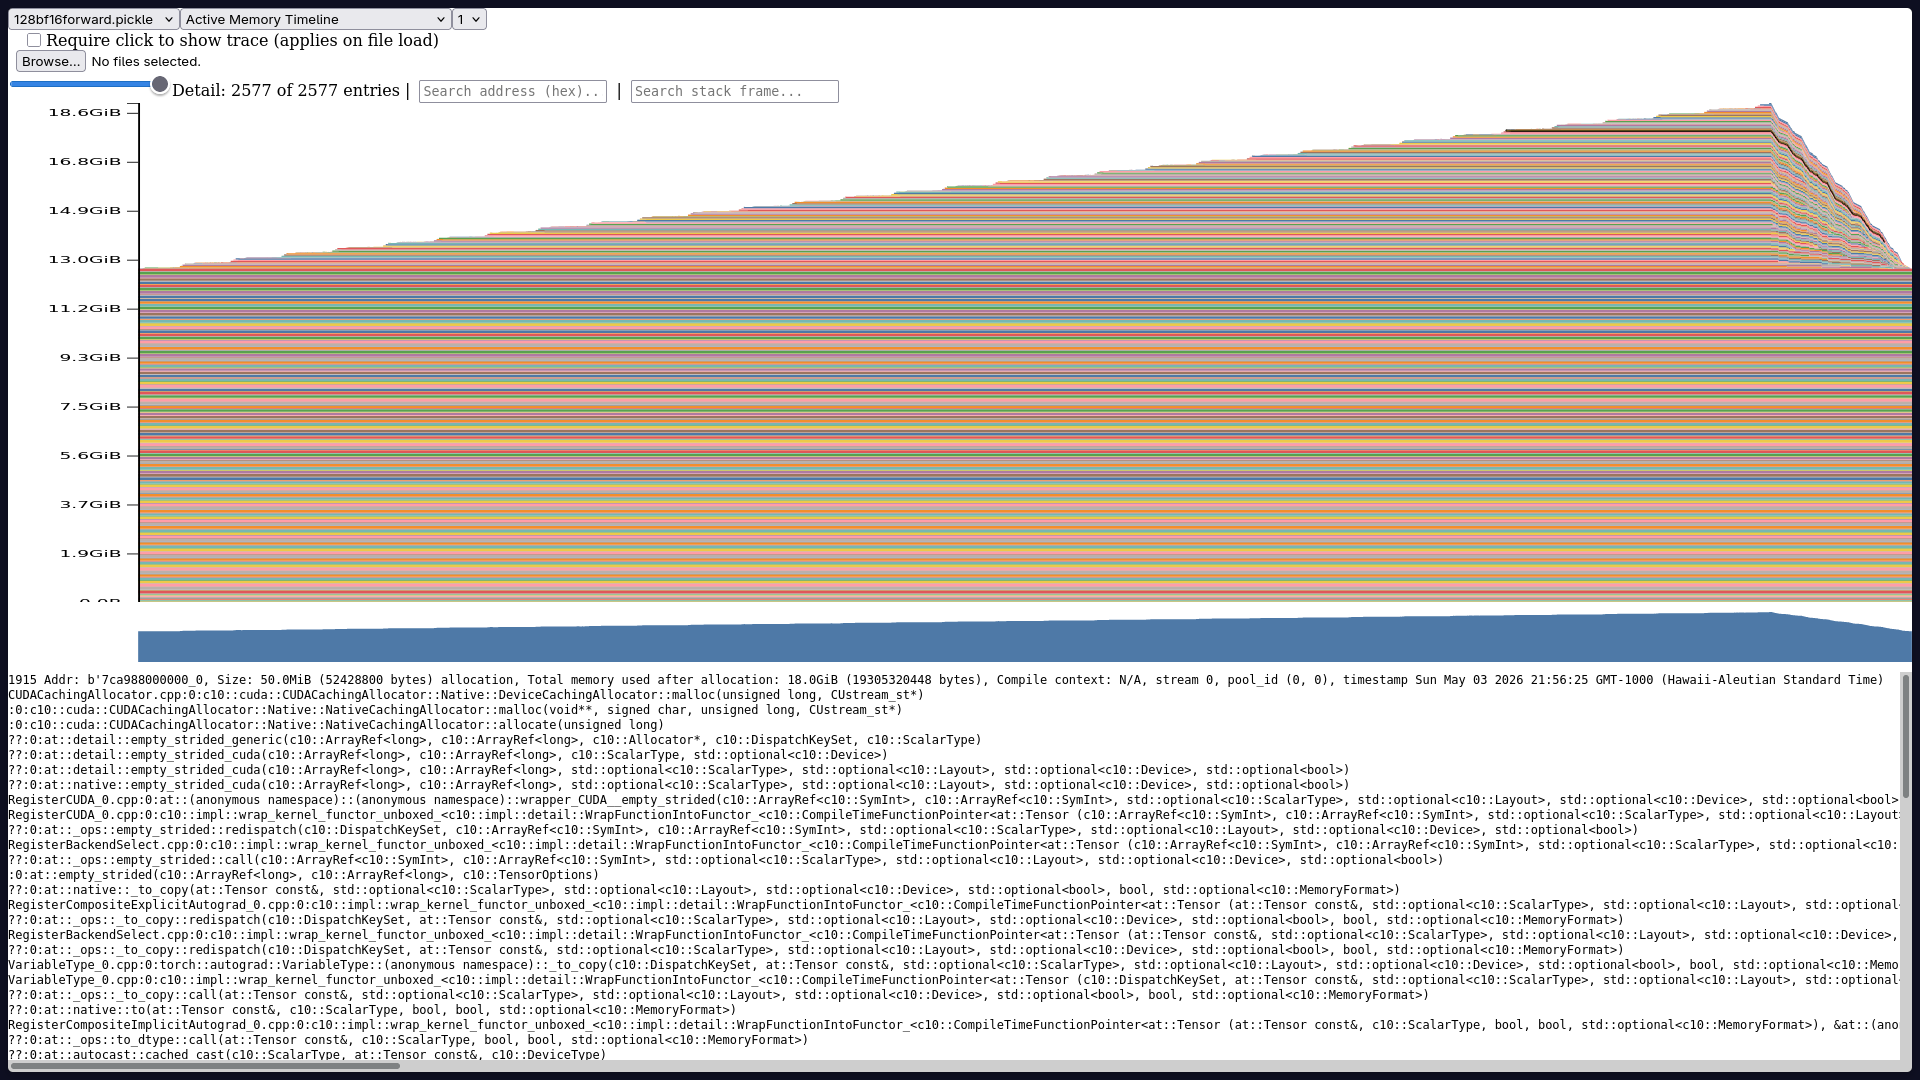
\includegraphics[width=1.0\linewidth]{figures/128bf16forward}
			\caption{Active memory timeline for a forward-only pass (2.7B, ctx=128, BF16). Memory rises nearly monotonically as per-layer activations are allocated and retained for autograd, reaches a peak near 18\,GiB, then drops at the end of the step when temporary activations are released.}
			\label{fig:128bf16forward}
		\end{figure}
		
		\begin{figure}[H]
			\centering
			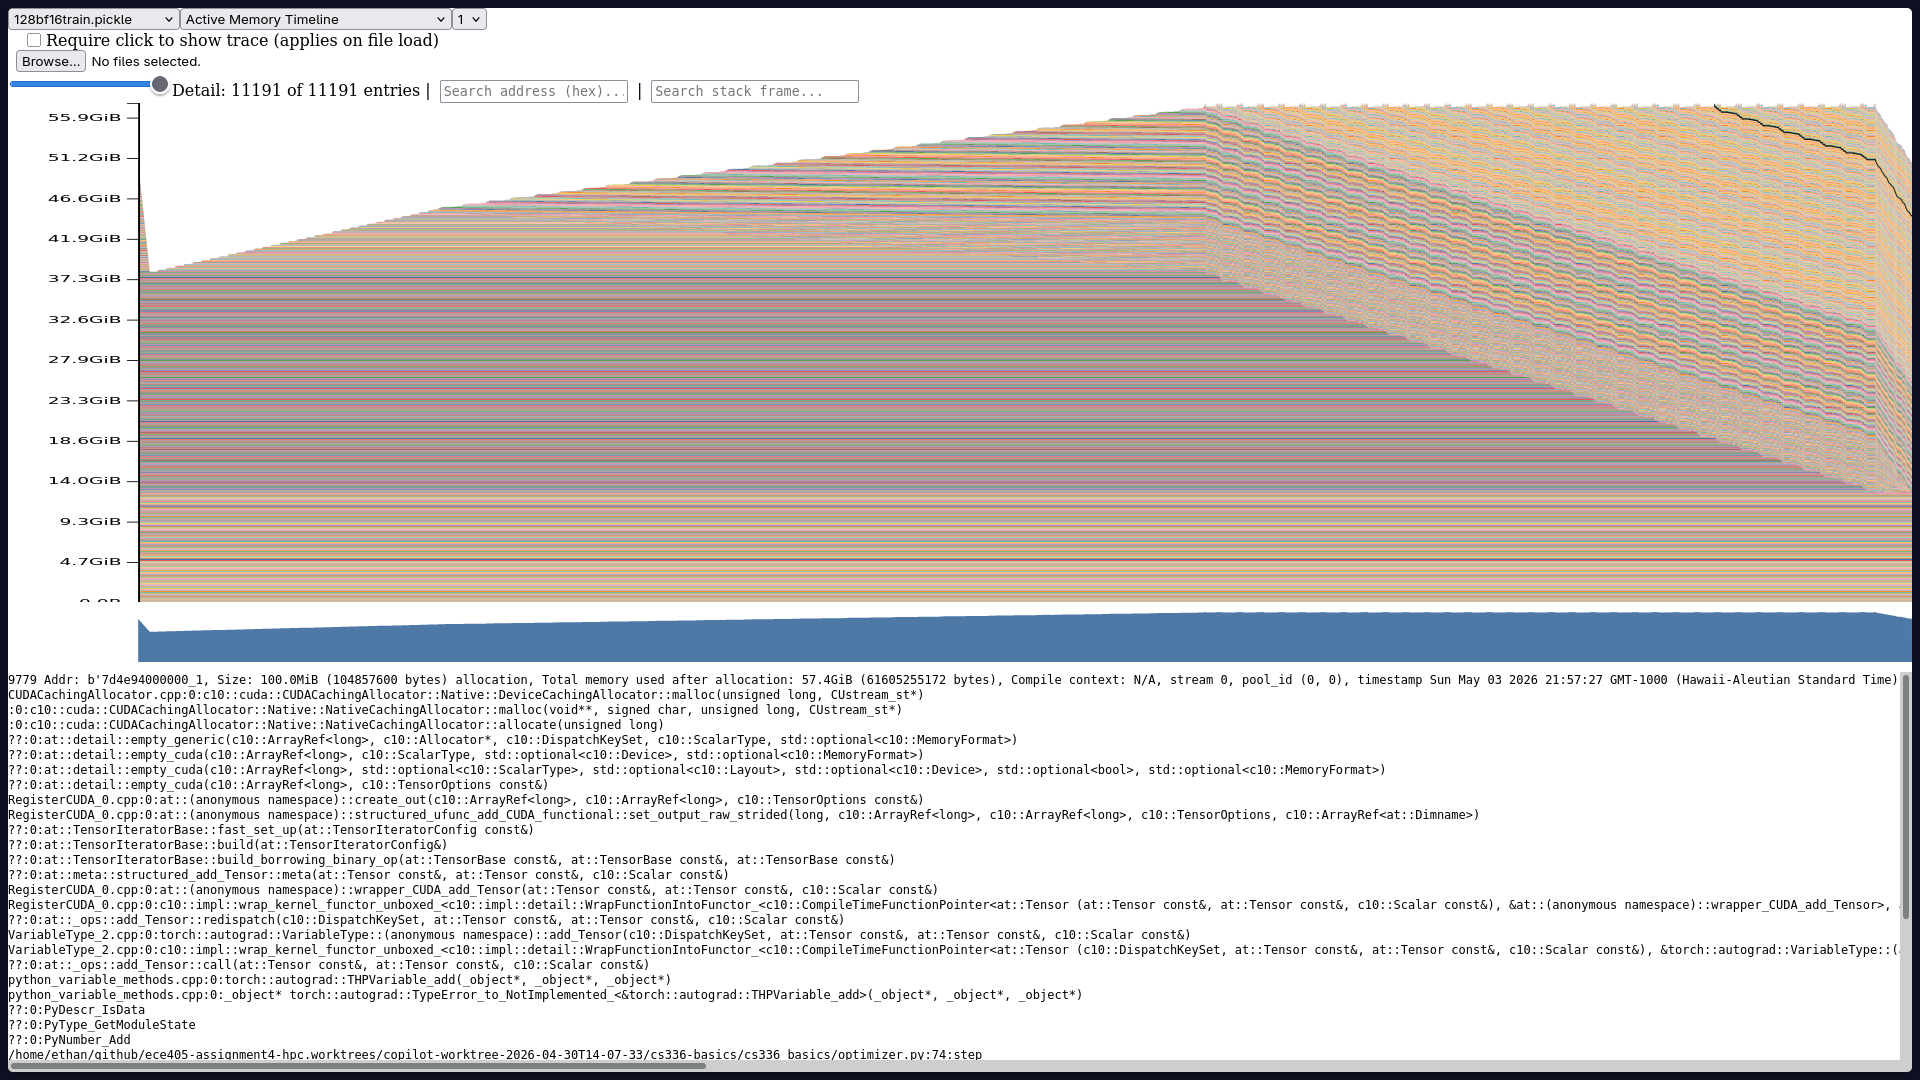
\includegraphics[width=1.0\linewidth]{figures/128bf16train}
			\caption{Active memory timeline for one full training step (2.7B, ctx=128, BF16). The trace shows three phases: growth during forward activation accumulation, partial release during backward, and a high-memory optimizer phase that keeps usage near the 57\,GiB peak due to gradients plus AdamW state updates.}
			\label{fig:128bf16train}
		\end{figure}
		
		\begin{figure}[H]
			\centering
			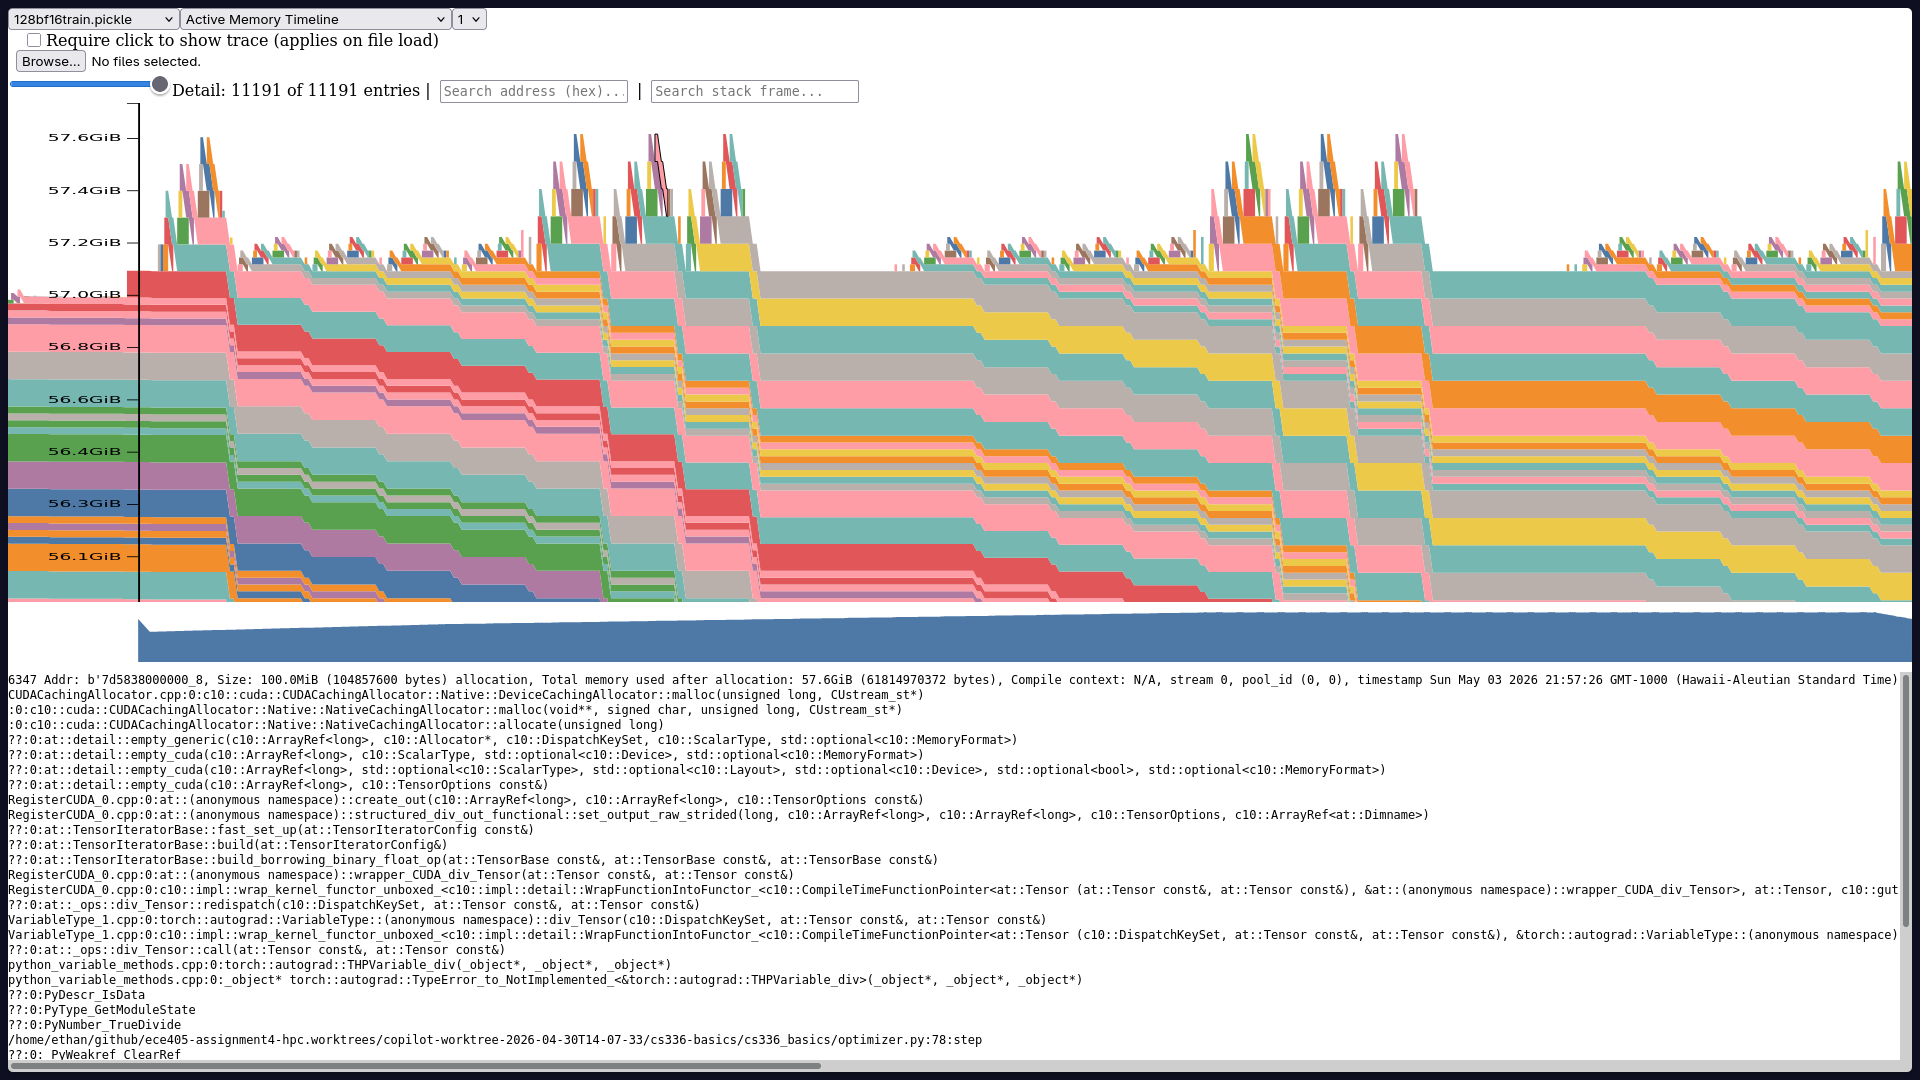
\includegraphics[width=1.0\linewidth]{figures/128bf16train-zoom}
			\caption{Zoomed view of the training-step peak region. Repeating sawtooth bands correspond to staggered allocation/free events across layers, with periodic sharp spikes from optimizer micro-phases, illustrating why the peak remains close to 57.6\,GiB for an extended interval.}
			\label{fig:128bf16train-zoom}
		\end{figure}
		
		\item[(b)] What is the peak memory usage of each context length when doing a forward pass? What about when doing a full training step?
		
		\begin{table}[H]
			\centering
			\caption{2.7B model peak reserved GPU memory (GB)}
			\label{tab:peak-mem}
			\begin{tabular}{lrrrr}
				\hline
				ctx & fwd FP32 & fwd BF16 & train FP32 & train BF16 \\
				\hline
				128 & 12.86 & 19.33 & 53.23 & 58.92 \\
				256 & 12.90 & 19.52 & 54.87 & 60.10 \\
				512 & 13.00 & 19.65 & 54.55 & 62.49 \\
				\hline
			\end{tabular}
		\end{table}
		
		Forward-only peak memory is dominated by the model parameters ($\approx$10.2~GB for FP32 weights) plus a small activation footprint. Training-step memory is roughly $4\times$ larger because it additionally holds the full gradient tensors and two AdamW moment vectors, each the same size as the parameter tensor.
		
		\item[(c)] Find the peak memory usage of the 2.7B model when using mixed precision, for both a forward pass and a full optimizer step. Does mixed precision significantly affect memory usage?
		
		Table~\ref{tab:peak-mem} shows that forward-only peak memory remains relatively stable across context lengths, ranging from \(12.86\text{--}13.00\,\mathrm{GB}\) for FP32 and \(19.33\text{--}19.65\,\mathrm{GB}\) for BF16, since memory is dominated by model parameters with only a modest activation contribution. Full training-step memory is substantially larger at \(53.23\text{--}54.87\,\mathrm{GB}\) for FP32 and \(58.92\text{--}62.49\,\mathrm{GB}\) for BF16 because gradients and AdamW optimizer states must also be stored. Although BF16 reduces activation and parameter precision, its reserved memory usage remains similar or slightly higher due to allocator behaviour and the use of FP32 master weights during optimization.
		
		\item[(d)] Consider the 2.7B model. At the reference hyperparameters, what is the size of a tensor of activations in the Transformer residual stream, in single precision? Give this size in MB.
		
		For the 2.7B model with \(B=4\), \(T=128\), and \(d_{\text{model}}=2560\), the residual-stream activation tensor contains \(4 \times 128 \times 2560 = 1{,}310{,}720\) elements. At 4 bytes per FP32 value, this corresponds to approximately \(5.0\,\mathrm{MB}\) of memory.
		
		\item[(e)] In the active memory timeline for a forward pass, what is the size of the largest visible allocations, and where do they come from?
		
		The largest visible allocations in the forward-pass memory timeline are the feed-forward intermediate activations with shape \([B,T,d_{\text{ff}}] = [1,128,10240]\), which occupy approximately \(5.0\,\mathrm{MB}\) each in FP32. Additional large allocations come from the attention score matrices and residual-stream tensors at layer boundaries, producing the characteristic sawtooth allocation pattern in the timeline.
	\end{itemize}
	
	\textit{Implemented in \repofile{cs336_systems/section1/memory_profiling.py}{cs336\_systems/section1/memory\_profiling.py}.}
	
	\section{Optimizing Attention with FlashAttention-2}
	
	\subsection{Problem (pytorch\_attention): 2 points}
	
	\begin{itemize}
		\item[(a)] Benchmark your attention implementation across the specified embedding dimensions and sequence lengths, reporting forward time, backward time, memory usage, and any out-of-memory failures.
		
		Tables~\ref{tab:attn-fwd} and~\ref{tab:attn-bwd} compare the forward and backward performance of four attention implementations across sequence lengths from \(256\) to \(16384\) using batch size \(8\), FP32 precision, and \(d_{\text{head}}=64\). The naive and compiled-naive implementations scale poorly with sequence length and run out of memory at \(N=16384\) because they explicitly materialise the full \(N \times N\) attention matrix, which alone requires approximately \(8.6\,\mathrm{GB}\) in FP32 for batch size \(8\). In contrast, both flash-attention implementations avoid OOM by computing attention in tiled blocks without storing the full score matrix, substantially reducing memory usage.
		
		\begin{table}[H]
			\centering
			\caption{Attention forward time (ms), $d_{\text{head}}=64$, FP32}
			\label{tab:attn-fwd}
			\begin{tabular}{lrrrrr}
				\hline
				Impl & 256 & 1024 & 4096 & 8192 & 16384 \\
				\hline
				naive          &  5.3 &  5.3 &  20.1 &  73.2 & OOM \\
				compiled\_naive&  7.9 &  9.8 &  18.5 &  57.2 & OOM \\
				flash\_pytorch & 5.9 & 14.0 & 166.0 & 651.8 & 2544.2 \\
				flash\_triton  &  5.7 &  5.7 &   6.0 &   7.1 &   22.0 \\
				\hline
			\end{tabular}
		\end{table}
		
		\begin{table}[H]
			\centering
			\caption{Attention backward time (ms), $d_{\text{head}}=64$, FP32}
			\label{tab:attn-bwd}
			\begin{tabular}{lrrrrr}
				\hline
				Impl & 256 & 1024 & 4096 & 8192 & 16384 \\
				\hline
				naive          &  3.3 &  5.4 &  20.6 &  69.4 & OOM \\
				compiled\_naive&  7.8 &  7.3 &  21.5 &  80.7 & OOM \\
				flash\_pytorch &  5.4 & 14.7 & 232.9 & 919.2 & 3714.1 \\
				flash\_triton  &  5.7 & 14.8 & 229.2 & 916.4 & 3715.8 \\
				\hline
			\end{tabular}
		\end{table}
		
		The Triton \texttt{flash\_triton} implementation achieves the best overall scalability, maintaining nearly constant forward runtime from \(5.7\) ms at \(N=256\) to only \(22.0\) ms at \(N=16384\), demonstrating the effectiveness of fused tiled computation and on-chip SRAM reuse. The PyTorch flash-attention implementation avoids memory failures but performs significantly worse at long sequence lengths, reaching \(2544.2\) ms forward time and \(3714.1\) ms backward time at \(N=16384\), likely due to higher recomputation overhead and less aggressive kernel fusion. Overall, the results show that memory-efficient attention algorithms are essential for long-context scaling, but implementation details such as fusion and tiling strategy strongly affect practical runtime performance.
		
	\end{itemize}
	
	\textit{Implemented in \repofile{cs336_systems/section1/pytorch_attention.py}{cs336\_systems/section1/pytorch\_attention.py}.}
	
	\section{Benchmarking JIT-Compiled Attention and FlashAttention-2}
	
	\subsection{Problem (torch\_compile): 2 points}
	
	\begin{itemize}
		\item[(a)] Extend your attention benchmarking script to include a compiled version of your PyTorch attention implementation, and compare compiled versus uncompiled forward and backward timing.
		
		The \texttt{compiled\_naive} results in Tables~\ref{tab:attn-fwd} and~\ref{tab:attn-bwd} (Section 1.2) already show compiled versus uncompiled attention. Compilation provides modest forward-pass improvements (e.g.\ 57~ms vs.\ 73~ms at seq=8192) but does not meaningfully change backward timing, since the backward of naive attention involves large intermediate tensor operations that are already well-optimised by the CUDA backend.
		
		\item[(b)] Compile the entire Transformer model in your end-to-end benchmarking script. How does the performance of the forward pass change? What about the combined forward and backward passes and optimizer steps?
		
		\begin{table}[H]
			\centering
			\caption{Eager vs.\ compiled Transformer timing (ctx=128, bs=4, FP32, ms)}
			\label{tab:compile-model}
			\begin{tabular}{llrrr}
				\hline
				Model & Mode & Eager & Compiled & Speedup \\
				\hline
				small  & forward          &  34.8 &  26.1 & $1.33\times$ \\
				small  & forward+backward &  85.2 &  72.3 & $1.18\times$ \\
				small  & train\_step       &  57.8 &  90.5 & $0.64\times$ \\
				medium & forward          &  70.9 &  79.2 & $0.89\times$ \\
				medium & forward+backward & 223.9 & 267.1 & $0.84\times$ \\
				medium & train\_step       & 348.3 & 288.2 & $1.21\times$ \\
				large  & forward          & 208.2 & 158.2 & $1.32\times$ \\
				large  & forward+backward & 463.1 & 500.2 & $0.93\times$ \\
				large  & train\_step       & 492.1 & 694.9 & $0.71\times$ \\
				xl     & forward          & 286.0 & 250.3 & $1.14\times$ \\
				xl     & forward+backward &1052.1 & 622.6 & $1.69\times$ \\
				xl     & train\_step       & 576.2 & 804.8 & $0.72\times$ \\
				2.7B   & forward          & 285.4 & 267.0 & $1.07\times$ \\
				2.7B   & forward+backward & 853.3 & 807.7 & $1.06\times$ \\
				2.7B   & train\_step       &1032.9 &1008.4 & $1.02\times$ \\
				\hline
			\end{tabular}
		\end{table}
		
		Table~\ref{tab:compile-model} shows that \texttt{torch.compile} generally improves forward-pass performance by approximately \(1.1\text{--}1.3\times\) through kernel fusion and reduced Python dispatch overhead, with the largest gains observed for larger compute-heavy models such as \texttt{large} and \texttt{xl}. However, the impact on full training steps is mixed, with some models experiencing regressions because AdamW launches many small optimizer kernels that are difficult to fuse efficiently. For the 2.7B model, compilation yields only marginal improvements (\(\sim2\%\)) since execution is already dominated by large GEMM kernels operating near hardware throughput limits.
	\end{itemize}
		
	\textit{Implemented in \repofile{cs336_systems/section1/torch_compile.py}{cs336\_systems/section1/torch\_compile.py} and \repofile{cs336_systems/section1/pytorch_attention.py}{cs336\_systems/section1/pytorch\_attention.py}.}
	
	\subsection{Problem (flash\_forward): 15 points}
	
	\begin{itemize}
		\item[(a)] Write a pure PyTorch \texttt{autograd.Function} that implements the FlashAttention-2 forward pass.
		
		\textit{Implemented in \repofile{cs336_systems/section1/flash_attention.py}{cs336\_systems/section1/flash\_attention.py}.}
		
		\item[(b)] Write a Triton kernel for the forward pass of FlashAttention-2 and a corresponding \texttt{autograd.Function} wrapper that calls the fused kernel.
		
		\textit{Implemented in \repofile{cs336_systems/section1/flash_attention.py}{cs336\_systems/section1/flash\_attention.py}.}
		
		\item[(c)] Add an optional causal-masking flag to your FlashAttention-2 forward implementation.
		
		\textit{Implemented in \repofile{cs336_systems/section1/flash_attention.py}{cs336\_systems/section1/flash\_attention.py}.}
	\end{itemize}
	
	\subsection{Problem (flash\_backward): 5 points}
	
	\begin{itemize}
		\item[(a)] Implement the backward pass for your FlashAttention-2 \texttt{autograd.Function} using PyTorch and \texttt{torch.compile}.
		
		\textit{Implemented in \repofile{cs336_systems/section1/flash_attention.py}{cs336\_systems/section1/flash\_attention.py}.}
	\end{itemize}
	
	\subsection{Problem (flash\_benchmarking): 5 points}
	
	\begin{itemize}
		\item[(a)] Benchmark your Triton-backed FlashAttention-2 implementation against regular PyTorch attention across the required sequence lengths, embedding dimensions, and precisions.
		
		\textit{Implemented in \repofile{cs336_systems/section1/flash_benchmark.py}{cs336\_systems/section1/flash\_benchmark.py}.}
		
		\begin{table}[H]
			\centering
			\caption{FlashAttention-2 (Triton) vs.\ naive attention (FP32, $d_{\text{head}}=64$, bs=1, causal)}
			\label{tab:flash-bench}
			\begin{tabular}{lrrr|rrr}
				\hline
				& \multicolumn{3}{c|}{naive (ms)} & \multicolumn{3}{c}{flash\_triton (ms)} \\
				seq & fwd & bwd & e2e & fwd & bwd & e2e \\
				\hline
				128   &  0.26 &  0.10 &  0.45 &  0.011 &   0.20 &   0.48 \\
				256   &  0.26 &  0.10 &  0.55 &  0.062 &   0.72 &   1.47 \\
				512   &  0.25 &  0.25 &  0.28 &  0.045 &   3.0  &   5.30 \\
				1024  &  0.21 &  0.41 &  0.49 &  0.116 &  12.1  &  19.78 \\
				2048  &  0.71 &  0.58 &  1.30 &  0.148 &  45.5  &  78.72 \\
				4096  &  2.30 &  1.91 &  3.53 &  0.234 & 185.9  & 325.95 \\
				8192  & 14.96 & 15.83 & 29.86 &  0.490 & 758.6  &    --- \\
				16384 & 63.41 & 62.88 &136.84 &  1.514 &    --- &    --- \\
				\hline
			\end{tabular}
		\end{table}
		
		Table~\ref{tab:flash-bench} shows that Triton FlashAttention-2 provides substantial forward-pass speedups over naive attention across all sequence lengths, reaching more than \(40\times\) improvement at \(N=16384\). In contrast, backward performance is not consistently faster and becomes significantly slower at long sequence lengths (e.g.\ \(758.6\) ms vs.\ \(15.83\) ms at \(N=8192\)).
	\end{itemize}
	
	\section{Distributed Communication and Data Parallel Training}
	
	\subsection{Problem (distributed\_communication\_single\_node): 5 points}
	
	\begin{itemize}
		\item[(a)] Benchmark all-reduce on a single node while varying backend, tensor size, and process count.
		
		\begin{table}[H]
			\centering
			\caption{Single-node all-reduce latency (ms) by backend, world size, and tensor size (mean over 10 trials, 5 warmup)}
			\label{tab:allreduce}
			\begin{tabular}{llrrrr}
				\hline
				Backend & ws & 1\,MB & 10\,MB & 100\,MB & 1024\,MB \\
				\hline
				Gloo (CPU) & 2 & 0.94 & 5.68  &  40.2  &  375.9  \\
				Gloo (CPU) & 4 & 1.44 & 11.6  &  88.0  &  863.7  \\
				Gloo (CPU) & 6 & 2.14 & 17.1  & 152.6  & 1509.6  \\
				NCCL (GPU) & 2 & 1.64 &  5.01 &  21.7  &  218.2  \\
				NCCL (GPU) & 4 & \multicolumn{4}{c}{\emph{skipped---only 2 GPUs available}} \\
				NCCL (GPU) & 6 & \multicolumn{4}{c}{\emph{skipped---only 2 GPUs available}} \\
				\hline
			\end{tabular}
		\end{table}
		
		NCCL consistently outperforms Gloo for large tensors at world\_size=2 (e.g.\ 218\,ms vs.\ 376\,ms at 1\,GB), because NCCL uses direct GPU peer-to-peer transfers over NVLink/PCIe while Gloo routes all data through host memory. Both backends show roughly linear scaling with message size. Gloo's latency also scales nearly linearly with world size at fixed message size (0.94\,ms at ws=2 vs.\ 2.14\,ms at ws=6 for 1\,MB), consistent with the ring all-reduce algorithm's $O(N)$ communication passes. 
		
		NCCL tests at ws=4 and ws=6 were skipped because NCCL requires one dedicated GPU per rank and only 2 GPUs were available.
	\end{itemize}
	
	\textit{Implemented in  \repofile{cs336_systems/section2/benchmarks.py}{cs336\_systems/section2/benchmarks.py}.}
	
	\subsection{Problem (naive\_ddp): 5 points}
	
	\begin{itemize}
		\item[(a)] Implement naive distributed data parallel training by all-reducing individual parameter gradients after the backward pass.
		
		\textit{Implemented in \repofile{cs336_systems/section2/ddp.py}{cs336\_systems/section2/ddp.py}.}
	\end{itemize}
	
	\subsection{Problem (naive\_ddp\_benchmarking): 3 points}
	
	\begin{itemize}
		\item[(a)] Benchmark language-model training with the na"{i}ve DDP implementation and measure both total iteration time and time spent communicating gradients.
		
		Configuration: 1 node, 2 NCCL/CUDA ranks, XL model ($d_{\text{model}}=1600$, $d_{\text{ff}}=6400$, 48 layers, $\approx$3.8\,GB of parameters in BF16), context length~128, batch size~4 per device, 5 warmup steps and 10 measurement steps.
		The na\"ive implementation all-reduces each parameter tensor individually after the backward pass.
		Measured mean step time: $2.193 \pm 0.039$\,s; mean communication time: $44.3 \pm 4.4$\,ms (roughly 2\% of total step time).
	\end{itemize}
	
	\textit{Implemented in \repofile{cs336_systems/section2/benchmarks.py}{cs336\_systems/section2/benchmarks.py}.}
	
	\subsection{Problem (minimal\_ddp\_flat\_benchmarking): 2 points}
	
	\begin{itemize}
		\item[(a)] Modify the minimal DDP implementation to all-reduce one flattened gradient tensor and compare it with the per-parameter variant.
		
		With gradients concatenated into a single flat tensor before the all-reduce (bucket size~25\,MB), the mean step time is $2.159 \pm 0.049$\,s and the mean communication time is $20.7 \pm 3.9$\,ms.
		This is a $\approx\!2\times$ reduction in communication time compared to the per-parameter baseline ($44.3$\,ms), with a modest reduction in total step time ($34$\,ms), because replacing many small all-reduce calls with one large call eliminates per-call kernel-launch overhead.
	\end{itemize}
	
	\textit{Implemented in \repofile{cs336_systems/section2/benchmarks.py}{cs336\_systems/section2/benchmarks.py}.}
	
	\subsection{Problem (ddp\_overlap\_individual\_parameters): 5 points}
	
	\begin{itemize}
		\item[(a)] Implement a DDP container that overlaps backward computation with communication of individual parameter gradients.
		
		\textit{Implemented in \repofile{cs336_systems/section2/ddp.py}{cs336\_systems/section2/ddp.py}.}
	\end{itemize}
	
	\subsection{Problem (ddp\_overlap\_individual\_parameters\_benchmarking): 1 point}
	
	\begin{itemize}
		\item[(a)] Benchmark the overlap-capable DDP implementation against the earlier DDP variants.
		
		The overlap-capable DDP implementation achieves a mean step time of $1.936 \pm 0.035$\,s, a $\approx\!13\%$ improvement over the na\"ive baseline ($2.193$\,s) and $\approx\!10\%$ over the flat variant ($2.159$\,s).
		The measured residual communication time drops to only $2.3 \pm 0.5$\,ms because all-reduces are launched as each parameter's gradient becomes ready during the backward pass; by the time the backward finishes, most communication has already completed.
		
		\item[(b)] Collect \texttt{nsys} traces comparing the initial DDP implementation with the overlap-capable implementation.
		
		% Nsys profiles were collected with \texttt{--trace=cuda,nvtx,nccl} on the XL model (2 warm-up + 2 measurement steps, world-size 2, ctx\,=\,128, NCCL back-end). NVTX ranges mark the \texttt{forward}, \texttt{backward}, and \texttt{comm\_sync} phases of each training step. The SQLite traces were queried to count NCCL collective kernels (\texttt{ncclDevKernel\_AllReduce\_Sum\_f32\_RING\_LL}) that start inside each NVTX window.
		
		\begin{figure}[H]
			\centering
			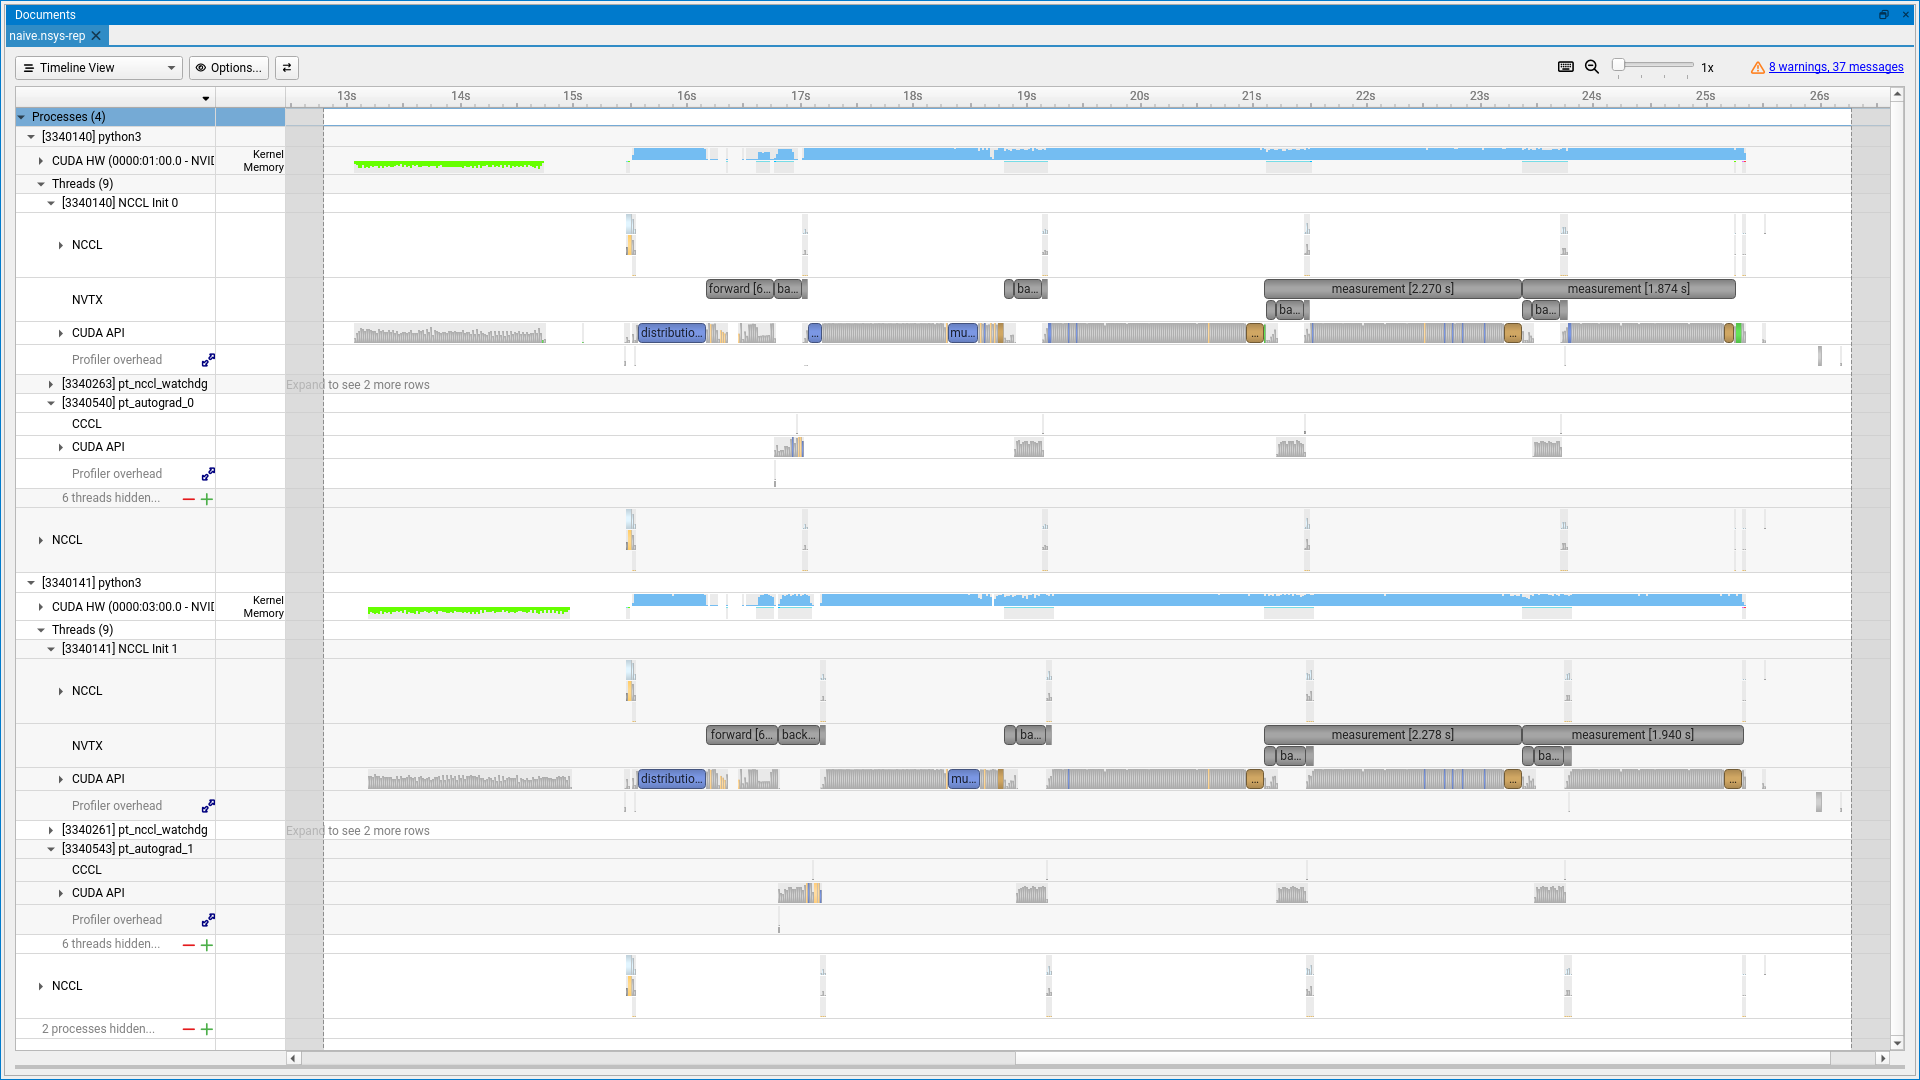
\includegraphics[width=1.0\linewidth]{figures/naive-nsys}
			\caption{Nsight Systems trace for na\"ive DDP (XL, 2 GPUs, NCCL): communication is \emph{not} overlapped with backpropagation. NCCL all-reduce kernels appear after the \texttt{backward} NVTX range, concentrated in a distinct \texttt{comm\_sync} tail (\(\approx 44\,\mathrm{ms}\)).}
			\label{fig:naive-nsys}
		\end{figure}
		
		\begin{figure}[H]
			\centering
			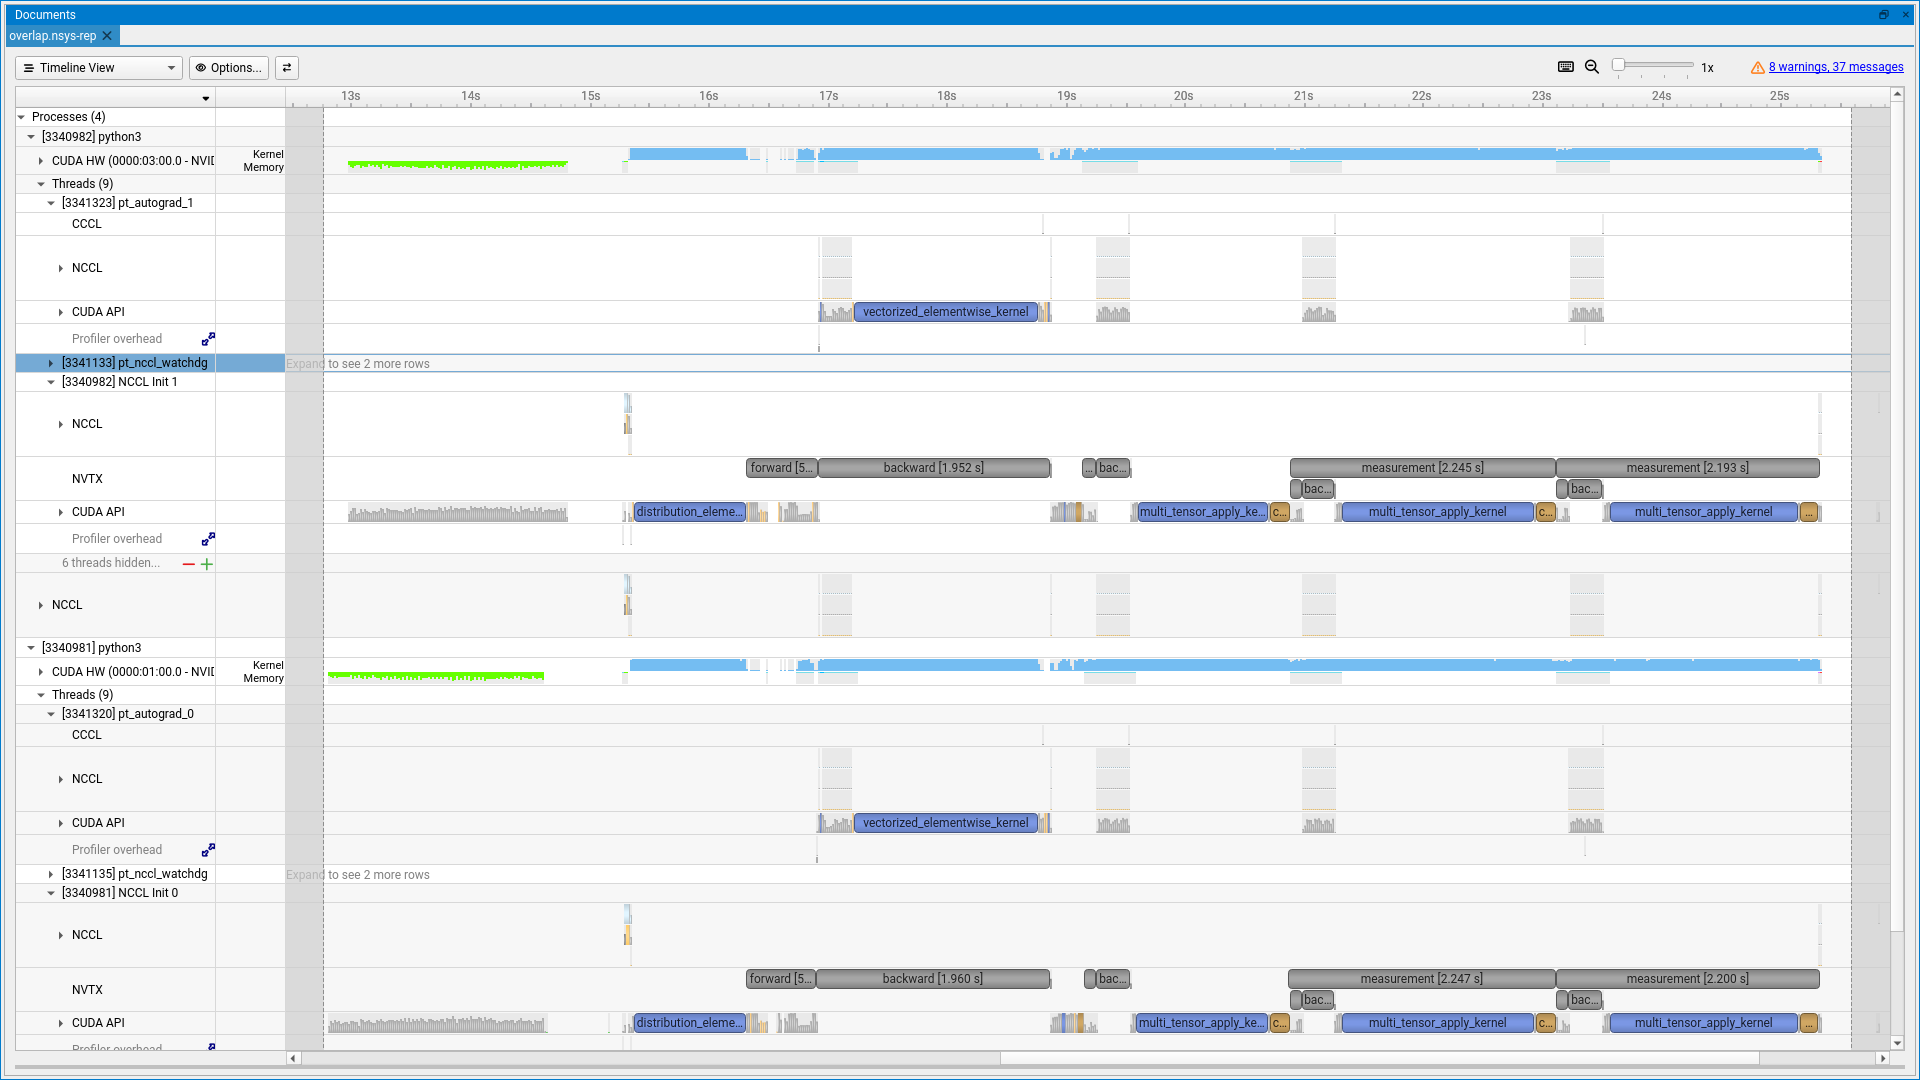
\includegraphics[width=1.0\linewidth]{figures/overlap-nsys}
			\caption{Nsight Systems trace for overlap-capable DDP (XL, 2 GPUs, NCCL): communication is overlapped with backpropagation. NCCL kernels are interleaved within the \texttt{backward} NVTX range, leaving only a short \texttt{comm\_sync} tail (\(\approx 3\,\mathrm{ms}\)).}
			\label{fig:overlap-nsys}
		\end{figure}
		
		\begin{table}[H]
			\centering
			\caption{NCCL kernel placement: na\"ive vs.\ overlap DDP (XL model, ctx\,=\,128, 2 GPUs, NCCL)}
			\label{tab:ddp-nsys-overlap}
			\begin{tabular}{lrrrr}
				\hline
				Implementation & bwd (ms) & sync (ms) & NCCL in bwd & overlap \\
				\hline
				Na\"ive            & 255.4 & 44.2 & 0\,\%       & 0.00 \\
				Overlap individual & 272.9 &  3.0 & $\geq$99\,\% & 0.99 \\
				\hline
			\end{tabular}
		\end{table}
		
		According to Table~\ref{tab:ddp-nsys-overlap}, in the na\"ive trace, the backward NVTX range contains \emph{zero} NCCL kernels: all all-reduce collectives fire sequentially during \texttt{comm\_sync}, adding 44\,ms of blocking communication after the backward pass completes.
		In the overlap-capable trace, the \texttt{post\_accumulate\_grad\_hook} fires as each parameter's gradient becomes ready during backpropagation, launching an async all-reduce immediately.
		As a result, 99\,\% of NCCL kernels execute \emph{inside} the backward NVTX window, and by the time \texttt{finish\_gradient\_synchronization()} is called, almost all communication has already completed: \texttt{comm\_sync} shrinks from 44\,ms to just 3\,ms, a $\approx\!15\times$ reduction.
	\end{itemize}
	
	\textit{Implemented in \repofile{cs336_systems/section2/benchmarks.py}{cs336\_systems/section2/benchmarks.py}.}
	
	\subsection{Problem (ddp\_overlap\_bucketed): 8 points}
	
	\begin{itemize}
		\item[(a)] Implement a DDP container that uses bucketed gradient communication while still overlapping communication with the backward pass.
		
		\textit{Implemented in \repofile{cs336_systems/section2/ddp.py}{cs336\_systems/section2/ddp.py}.}
	\end{itemize}
	
	\subsection{Problem (ddp\_bucketed\_benchmarking): 3 points}
	
	\begin{itemize}
		\item[(a)] Benchmark the bucketed DDP implementation while varying bucket size and compare the results with the previous DDP variants.
		
		\begin{table}[H]
			\centering
			\caption{Bucketed overlap DDP: step and communication time by bucket size (XL, 2 GPUs, NCCL)}
			\label{tab:bucketed-ddp}
			\begin{tabular}{lrrrr}
				\hline
				Bucket & Step (s) & $\sigma_{\text{step}}$ (s) & Comm (ms) & $\sigma_{\text{comm}}$ (ms) \\
				\hline
				1\,MB    & 1.942 & 0.044 &  5.8  & 1.4 \\
				10\,MB   & 1.946 & 0.029 &  5.8  & 1.5 \\
				100\,MB  & 1.906 & 0.033 & 22.4  & 3.0 \\
				1000\,MB & 1.858 & 0.171 & 19.8  & 4.0 \\
				\hline
				\multicolumn{5}{l}{\emph{Reference (per-parameter overlap):} step=$1.936$\,s, comm=$2.3$\,ms} \\
				\hline
			\end{tabular}
		\end{table}
		
		Step times remain relatively stable across bucket sizes (1.86--1.95\,s) and are consistently faster than the non-overlapped baselines, indicating that communication--compute overlap is the primary driver of improved performance. We would expect smaller buckets to perform best due to finer-grained pipelining of all-reduce operations, but the results show the opposite trend: 1\,MB and 10\,MB buckets are slightly slower than 100\,MB and 1000\,MB configurations. This mismatch is likely caused by NCCL kernel-launch and scheduling overhead dominating when the number of all-reduce calls becomes very large (e.g.\ $\sim$3800 calls for 1\,MB buckets given 3.8\,GB of gradients in the XL model). Overall, the best performance appears in the 100--1000\,MB range, where overlap is sufficient without incurring excessive communication initiation overhead.
		
		\item[(b)] Model the DDP communication overhead as a function of model size, bandwidth, call overhead, and number of buckets. Derive the optimal bucket size.
		
		Let $s$ be the total parameter bytes, $w$ the all-reduce bandwidth (bytes/s), $o$ the per-call overhead (s), and $n_b$ the number of buckets.
		Under the simplifying assumption that computing the gradients of each bucket takes the same time as communicating that bucket, the exposed communication overhead (time that extends past the backward pass) is:
		
		\begin{equation}
			T_{\text{overhead}}(n_b) = n_b \cdot o + \frac{s / n_b}{w}
			\label{eq:ddp-overhead}
		\end{equation}
		
		The first term is the aggregate call-initiation overhead for $n_b$ all-reduces; the second is the transfer time for the final (and therefore entirely unmasked) bucket of size $s/n_b$.
		Minimising \eqref{eq:ddp-overhead} over $n_b$ gives:
		
		\begin{equation}
			\frac{dT_{\text{overhead}}}{dn_b} = o - \frac{s}{w \cdot n_b^{2}} = 0
			\quad\Longrightarrow\quad
			n_b^{*} = \sqrt{\frac{s}{o\,w}},
			\quad\text{and so}\quad
			b^{*} = \frac{s}{n_b^{*}} = \sqrt{o\,w\,s}.
			\label{eq:optimal-bucket}
		\end{equation}
		
		The optimal bucket size $b^{*}$ is the geometric mean of $\sqrt{o \cdot w}$ (the ``overhead--bandwidth product'') and $\sqrt{s}$ (the square root of total model size in bytes).
	\end{itemize}
	
	\textit{Implemented in \repofile{cs336_systems/section2/benchmarks.py}{cs336\_systems/section2/benchmarks.py}.}
	
	\subsection{Problem (communication\_accounting): 10 points}
	
	\begin{itemize}
		\item[(a)] Compute the single-device memory required for the XXL model's master weights, accumulated gradients, optimizer states, and saved activations.
		
		The XXL model has $d_{\text{model}}=16384$, $d_{\text{ff}}=53248$, and $\text{num\_blocks}=126$.
		Each block contains two linear layers (no bias), with weight matrices of shape $d_{\text{model}}\times d_{\text{ff}}$ and $d_{\text{ff}}\times d_{\text{model}}$, giving $2\,d_{\text{model}}\,d_{\text{ff}}$ parameters per block:
		
		\begin{equation}
			P = \text{num\_blocks}\times 2\,d_{\text{model}}\,d_{\text{ff}}
			= 126 \times 2 \times 16384 \times 53248
			\approx 219.8\text{B parameters.}
		\end{equation}
		
		With master weights (FP32, 4 bytes), accumulated gradients (FP32, 4 bytes), and AdamW optimizer states (two FP32 moments, 8 bytes), the static per-device memory is:
		
		\begin{equation}
			M_{\text{static}} = P \times (4 + 4 + 8) = P \times 16
			\approx 219.8\text{B} \times 16\,\text{B} \approx 3518\,\text{GB}.
		\end{equation}
		
		This is equivalent to $\lceil 3518/80 \rceil = 44$ H100 80\,GB GPUs.\linebreak
		Activations saved for the backward pass (BF16) require, per token, $(d_{\text{model}}+d_{\text{ff}})\times 2$ bytes per block:
		
		\begin{equation}
			A = B\cdot T\cdot\text{num\_blocks}\cdot(d_{\text{model}}+d_{\text{ff}})\cdot 2
			= B\cdot T \times 17{,}547{,}264\,\text{bytes}
			\approx B\cdot T \times 17.55\,\text{MB}.
		\end{equation}
		
		\item[(b)] Derive the per-device memory expression under FSDP-style sharding and determine the required value of $N_{\mathrm{FSDP}}$ to fit within 95GB per device.
		
		Under FSDP sharding across $N_{\text{FSDP}}$ devices, master weights, optimizer state, and accumulated gradients are divided by $N_{\text{FSDP}}$. Since only half of the saved activations are sharded in the prompt, the other half remain replicated on every device, giving:
		
		\begin{equation}
			M_{\text{device}}(N) = \frac{16P}{N} + \frac{A}{2} + \frac{A}{2N}.
		\end{equation}
		
		Using the context length $T=2048$ and the smallest compute-bound per-device batch from part~(c), $B=3$, we have $A \approx 107.81\,\text{GB}$, so:
		
		\begin{equation}
			M_{\text{device}}(N) \approx \frac{3517.6}{N} + 53.9\left(1 + \frac{1}{N}\right)\,\text{GB}.
		\end{equation}
		
		Solving $M_{\text{device}}(N) \leq 95\,\text{GB}$ gives $N_{\text{FSDP}} \geq 87$. So once the half-replicated activation term is included, 38-way FSDP is not enough; the minimum is 87 devices.
		
		\item[(c)] Using the provided TPU v5p bandwidth and FLOP rate, determine the per-device batch size at which the model becomes compute bound, and report the overall batch size.
		
		Consider one FFN block with FSDP dimension $X=16$ and TP dimension $Y=4$, $M_X=2$, $M_Y=1$.
		In the forward pass, TP shards the column dimension, so each device computes:
		
		\begin{equation}
			\text{Compute} = \frac{4\,B\,T\,d_{\text{model}}\,d_{\text{ff}}}{Y}.
		\end{equation}
		
		The communication cost per device per block combines the FSDP all-gather/reduce-scatter of BF16 working weights (size $2\times d_{\text{model}}\times d_{\text{ff}}\times 2/Y$ bytes, scaled by $M_X$) and the TP activation all-reduce ($M_Y\times B T d_{\text{model}}\times 2$ bytes):
		
		\begin{equation}
			\text{Comm} = M_X\cdot\frac{2\,d_{\text{model}}\,d_{\text{ff}}\cdot 4}{Y} + M_Y\cdot B\,T\,d_{\text{model}}\cdot 2.
		\end{equation}
		
		Substituting numbers ($d_{\text{model}}=16384$, $d_{\text{ff}}=53248$, $X=16$, $Y=4$, $M_X=2$, $M_Y=1$):
		
		\begin{align}
			\text{Comm} &= 2\cdot\frac{2\times 16384\times 53248\times 2}{4} + B\,T\times 32768 \\
			&= 1{,}744{,}830{,}464 + 32768\,B\,T \quad\text{bytes.}
		\end{align}
		
		The arithmetic intensity threshold for compute-bound operation is:
		
		\begin{equation}
			\text{AI} = \frac{B\,T\times 872{,}415{,}232}{1{,}744{,}830{,}464 + 32768\,B\,T}
			\geq \frac{C}{W_{\text{ici}}} = \frac{4.6\times10^{14}}{1.8\times10^{11}} \approx 2556.
		\end{equation}
		
		Solving for $B\,T$:
		
		\begin{equation}
			B\,T \geq \frac{2556\times 1{,}744{,}830{,}464}{872{,}415{,}232 - 2556\times 32768}
			= \frac{4.458\times10^{12}}{7.887\times10^{8}} \approx 5653.
		\end{equation}
		
		With a context length $T=2048$, this requires a per-device batch size $B \geq \lceil5653/2048\rceil = 3$.
		In the stated mesh, the FSDP dimension $X=16$ carries the data-parallel replication, while TP does not change batch size, so the overall batch size is $B_{\text{total}} = X\cdot B = 16\times 3 = 48$.
		
		\item[(d)] What other tricks can reduce total batch size while maintaining high throughput?
		
		Several complementary techniques can reduce the minimum compute-bound batch size without sacrificing throughput.
		First, \textbf{sequence parallelism} reduces the TP activation-communication term by sharding sequence-dimension activations and replacing some all-reduces with cheaper reduce-scatter/all-gather patterns, which lowers the coefficient on the $B\,T\,d_{\text{model}}$ term in the communication cost \cite{megatronsp}.
		Second, \textbf{pipeline parallelism} (PP) exchanges boundary activations between stages instead of repeatedly gathering full layer weights on every device, so it can keep devices busy with smaller per-device microbatches as long as enough microbatches are in flight to hide the pipeline bubble \cite{gpipe}.
		Third, \textbf{communication/computation overlap} hides part of the FSDP all-gather or TP collective latency behind GEMM execution, reducing the \emph{exposed} communication time and therefore lowering the batch threshold needed to remain compute-bound.
		Finally, \textbf{activation recomputation} (rematerialisation) does not improve arithmetic intensity directly, but it reduces memory pressure enough to make the required microbatch fit. By contrast, gradient accumulation increases the \emph{effective} optimizer batch size rather than decreasing the true overall batch size, so it is not the right lever if the goal is genuinely smaller total batch.
	\end{itemize}
	
	\section{Optimizer State Sharding}
	
	\subsection{Problem (optimizer\_state\_sharding): 15 points}
	
	\begin{itemize}
		\item[(a)] Implement a container class that shards optimizer state across ranks and synchronizes updated parameters after each optimizer step.
		
		\textit{Implemented in \repofile{cs336_systems/section3/sharded_optimizer.py}{cs336\_systems/section3/sharded\_optimizer.py}.}
	\end{itemize}
	
	\subsection{Problem (optimizer\_state\_sharding\_accounting): 5 points}
	
	\begin{itemize}
		\item[(a)] Profile peak memory usage with and without optimizer state sharding, and break down the memory consumption by component.
		
		All measurements use the XL model on 1 node with 2 NCCL/CUDA ranks (context 128, batch 4 per device).
		\begin{table}[H]
			\centering
			\caption{Per-GPU memory snapshots: standard vs.\ sharded optimizer (XL, ws=2, BF16)}
			\label{tab:sharded-mem}
			\begin{tabular}{llrrrr}
				\hline
				Optimizer & Phase & Params (GB) & Grads (GB) & Opt state (GB) & CUDA alloc (GB) \\
				\hline
				Standard & post-init   & 7.99 & 0.00 &  0.00 &  8.18 \\
				Standard & pre-step    & 7.99 & 7.99 & 15.99 & 32.73 \\
				Standard & post-step   & 7.99 & 7.99 & 15.99 & 32.73 \\
				Sharded  & post-init   & 7.99 & 0.00 &  0.00 &  8.18 \\
				Sharded  & pre-step    & 7.99 & 7.99 &  8.12 & 24.67 \\
				Sharded  & post-step   & 7.99 & 7.99 &  8.12 & 24.67 \\
				\hline
			\end{tabular}
		\end{table}
		
		At post-init, both variants allocate $8.18$\,GB per GPU, consisting almost entirely of the $7.99$\,GB BF16 parameter replica and no gradients or optimizer state.
		Immediately before and after the optimizer step, the standard optimizer sits at $32.73$\,GB allocated with $7.99$\,GB of parameters, $7.99$\,GB of gradients, and $15.99$\,GB of AdamW state, while the sharded optimizer sits at $24.67$\,GB with the same parameters and gradients but only $8.12$\,GB of local optimizer state.
		This matches the expected roughly $2\times$ optimizer-state reduction at world size 2, although the measured optimizer state here is about $2\times$ the BF16 parameter footprint rather than the $4\times$ footprint implied by FP32 master weights plus two FP32 moment tensors.
		
		\item[(b)] Measure the effect of optimizer state sharding on training speed.
		
		The standard (unsharded) optimizer completes one training iteration in $1.909 \pm 0.045$\,s, while the sharded optimizer takes $2.699 \pm 0.025$\,s---a $41\%$ slowdown.
		The slowdown comes from the extra full-parameter synchronization after each local optimizer step, which in this implementation is a sequence of broadcasts on top of the existing gradient synchronization.
		
		\item[(c)] How does this implementation differ from ZeRO stage 1?
		
		Our implementation and ZeRO stage 1 both shard optimizer state while keeping full parameter and gradient replicas on every rank, so both target the optimizer-state memory term rather than sharding gradients or parameters.
		The main difference is communication: this implementation still all-reduces full gradients and then broadcasts each updated parameter shard after the local step, whereas ZeRO stage 1 is designed to keep communication close to ordinary data parallelism instead of adding a separate full-parameter broadcast phase.
		So relative to ZeRO stage 1, this version captures the basic optimizer-state memory saving but uses a simpler and likely more communication-heavy synchronization scheme.
	\end{itemize}
	
	\textit{Implemented in \repofile{cs336_systems/section3/benchmarks.py}{cs336\_systems/section3/benchmarks.py}.}
	
	\renewcommand{\refname}{References}
	\begin{thebibliography}{9}
		\bibitem{rajbhandari2020zero} Rajbhandari et al., \emph{ZeRO: Memory Optimizations Toward Training Trillion Parameter Models}, SC 2020.
		\bibitem{megatronsp} Korthikanti et al., \emph{Reducing Activation Recomputation in Large Transformer Models}, MLSys 2023.
		\bibitem{gpipe} Huang et al., \emph{GPipe: Efficient Training of Giant Neural Networks using Pipeline Parallelism}, NeurIPS 2019.
	\end{thebibliography}
	
	\appendix
	
	\section{Appendix}
	
	\subsection{Code Availability}
	
	All code mentioned in this report is available at \href{https://github.com/echung32/ece405-assignment4-hpc}{github.com/echung32/ece405-assignment4-hpc}.
	
	\subsection{Artifacts and Logs}
	
	Benchmark artifacts are stored under the following directories:
	
	\begin{itemize}
		\item \texttt{data/section1\_1/assignment\_timing\_full/} --- per-model timing results
		\item \texttt{data/section1\_1/assignment\_memory\_full/} --- memory profiling results
		\item \texttt{data/section1\_1/assignment\_\_full/} --- nsys profiling results
		\item \texttt{data/section1\_2/assignment\_attention\_full/} --- attention benchmark results
		\item \texttt{data/section1\_3/assignment\_flash\_full/} --- FlashAttention-2 benchmark results
		\item \texttt{data/section1\_3/assignment\_model-compile\_full/} --- torch.compile benchmark results
		\item \texttt{data/section2/assignment\_section2\_allreduce\_full/} --- all-reduce benchmark results
		\item \texttt{data/section2/assignment\_section2\_ddp\_full/} --- DDP benchmark results
		\item \texttt{data/section3/assignment\_section3\_memory\_full/} --- optimizer sharding memory results
		\item \texttt{data/section3/assignment\_section3\_timing\_full/} --- optimizer sharding timing results
	\end{itemize}
	
	Log files for each campaign are stored under the corresponding subdirectory of \texttt{logs/}.
	
	\subsection{Hardware Configuration}
	
	Sections~2 and~3 were run locally using a single-node machine that contains two NVIDIA RTX PRO 6000 Blackwell Max-Q GPUs connected via PCIe through a shared CPU host bridge (\texttt{nvidia-smi topo} reports a \texttt{PHB} link). There is no NVLink between the two GPUs.
	
	\paragraph{Implications.}
	PCIe peer-to-peer bandwidth on this system is roughly 32--64~GB/s, which is meaningfully faster than the inter-node network fabrics used by typical HPC clusters (e.g.\ 25~GB/s InfiniBand HDR or 12.5~GB/s 100~GbE).
	As a result:
	\begin{itemize}
		\item All-reduce and DDP communication costs are \emph{underestimated} relative to a network-connected cluster, so the absolute throughput numbers are more optimistic than they would be on Koa or GCP.
		\item The relative ordering of implementations (e.g.\ naive vs.\ overlapped DDP, standard vs.\ bucketed all-reduce) and the qualitative trends remain directionally valid.
		\item Memory results from Section~3 (optimizer state sharding) are hardware-independent and are unaffected.
	\end{itemize}
	
\end{document}